\chapter{Design}
\label{chapter:design}
   The purpose of this chapter is to document design decisions for Haar and the underlying Haar Engine. It is an important stage in the development of these system components because it combines the requirements specified in Chapter \ref{Chapter:Specification} and the knowledge gained in Chapter \ref{Chapter:Background}. The process has been highly iterative and has led to the upcoming system architecture. 

   One fact which has become clear throughout the design process is that the design and implementation are not mutually exclusive. Some ideas presented in Chapter \ref{Chapter:Background} are dependant on specific technologies, such as the ability to facilitate bidirectional communication (Section \ref{bidirectioncomms}). For this project, the available tools and technologies have therefore informed the design, and this has been integrated to the design process.

   The design process for each functional requirement has consisted of three iterative stages, as shown in Figure \ref{figure:design-process}. First of all, the initial research is consulted to check if any knowledge could inform the design. The requirement and existing knowledge were then used as a basis as a small feasibility investigation for various technologies. Based on these findings, the design was updated. This process was repeated for individual requirements, as well as between requirements to ensure the complete system will operate adequately.

   \begin{figure}
    \centering
      \begin{tikzpicture}
        \node[align=center] at (5.5,5) {Update Design};
        \draw (3.5,4) rectangle (7.5,6);

        \node[align=center] at (2,1) {Implementation\\Feasibility};
        \draw (0,0) rectangle (4,2);

        \node[align=center] at (9,1) {Reflect on\\Research};
        \draw (7,0) rectangle (11,2);

        \path (2,2) edge [->,thick,out=100,in=190]  (3.5,5);
        \path (7.5,5) edge [->,thick,out=350,in=80]  (9,2);
        \path (7,1) edge [->,thick,out=190,in=350]  (4,1);
      \end{tikzpicture}
    \caption{Iterative steps when designing for functional requirements}\label{figure:design-process}
  \end{figure}

  \section{Haar Engine}
    The first component to get design attention is the Haar Engine. The purpose of this framework is to provide the tools which enable developers to implement an IoT application. Since this will support the main system functions required for an IoT system applications, its design is heavily informed by the technologies available.

    One major design decision is the programming environment used to implement the Haar Engine. First of all, the chosen programming language and ecosystem must be able to support the requirements outlined in the previous chapter. Beyond that, the language and framework must provide suitable constructs so application developers can easily extend and modify for their own needs. Various languages and architectures were investigated (such as PHP, Ruby, Python and Go), however one stood out as being most suitable for this project, given the constraints: server-side JavaScript in the form of Node.js.

    JavaScript and the Node.js ecosystem will be discussed in greater detail in the implementation chapter, however there are some language features which are pertinent to the design of the framework. First of all, JavaScript is a weakly-typed, dynamic programming language. It does not support interfaces or abstract classes like Java, and variables are not defined with strict values. Care should therefore be taken when modelling system components as objects. JavaScript itself operates using the so-called event loop and all operations are considered asynchronous. Care should therefore be given to function executions, callbacks and the required call order.

    Node.js is a server-side implementation of the Google V8 JavaScript engine and it provides a programming API. There are various web application frameworks developed on top of Node.js, with the de facto standard being Express. The Express framework is based on the concept of middleware, where middleware functions anonymously pass objects to the next one until a web request has been finished. This concept could therefore be used to an advantage for system aspects like authentication.

    Bearing these language features in mind, a final design for the framework has been defined. A logical view of the main system components can be seen in Figure \ref{figure:framework-architecture}. The design decisions for each of these framework components have been described in the following subsections.

    \begin{figure}
    \centering
      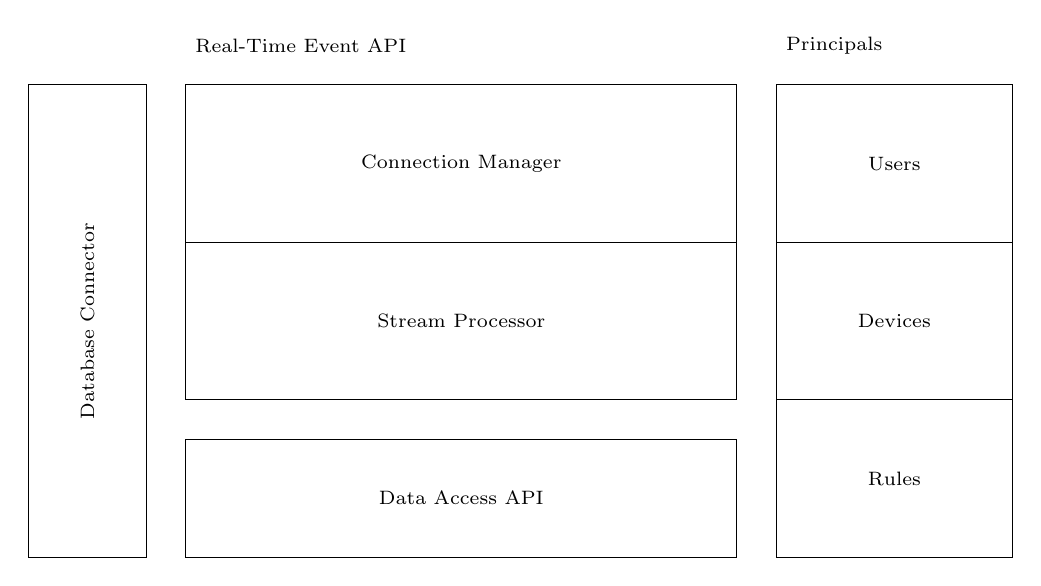
\begin{tikzpicture}
        \draw (0,0) rectangle (1.5,6);
        \node[align=center, rotate=90] at (0.75,3) {Database Connector};

        \draw (2,2) rectangle (9,6);
        \draw (2,4) -- (9,4);
        \node[anchor=west] at (2,6.5) {Real-Time Event API};
        \node[align=center] at (5.5,5) {Connection Manager};
        \node[align=center] at (5.5,3) {Stream Processor};

        \draw (2,0) rectangle (9,1.5);
        \node[align=center] at (5.5,0.75) {Data Access API};

        \draw (9.5,0) rectangle (12.5,6);
        \draw (9.5,4) -- (12.5,4);
        \draw (9.5,2) -- (12.5,2);
        \node[anchor=west] at (9.5,6.5) {Principals};
        \node[align=center] at (11,5) {Users};
        \node[align=center] at (11,3) {Devices};
        \node[align=center] at (11,1) {Rules};
      \end{tikzpicture}
    \caption{A logical view of system architecture for the Haar Engine}\label{figure:framework-architecture}
  \end{figure}

    \subsection{Data Modelling}
      The functional requirements in Chapter \ref{Chapter:Specification} make reference to a number of modellable objects. In particular these are users, devices and rules, and they all have a notion of ownership and authorisation within the framework. During initial research, it was found that an existing platform (Nitrogen.io) abstracts similar objects into a collection called principals. Throughout the design process, users, devices and rules have have proven to be first-class citizens of the framework, so the Haar Engine will adopt the same terminology.

      The three principal objects set foundations for the complete data model as well as other framework components, so it is important that they are modelled correctly. This subsection will first describe the traits of each principle before expanding their relationships into an entity-relationship model. Figure \ref{figure:principal-models} illustrates the relationship between the principals.

      \subsubsection{Users}
        The user principal is fundamentally responsible for authorisation within the Haar Engine. This will model an end-user account such as an individual person or a company, who will access their account using a unique username and a password. The user is responsible for managing their own devices and rules. The Haar Engine will identify user principals with a unique identifier. This would allow users to change their username while maintain relationships with other principals.

        User principals will be the gatekeeper to devices associated with their account. First of all, they will be able to attach new devices to their account. Users will also have the ability to share access to sensor devices with specific users, or make that data publicly available. Finally, user principals will have the ability to transfer ownership of the device to another Haar Engine user account and relinquish administration control over it.

        User principals will also be able to create, modify and delete rules. When a new rule is created, the user will be designated as the owner of it. Unlike devices, users cannot share rules with another user, nor can they transfer ownership. It is foreseeable that a rule is configured to watch sensor data which is owner by another user. Since access to a third-party sensor cannot be granted, the rule would not have appropriate access permissions to run.

      \subsubsection{Devices}
        The device principal will model a single IoT device. The device can be one of two types (either a sensor or an actuator). Devices will be owned by one user, however further users may be granted access to access sensor data. Devices will be identifiable with a unique identifier in the Haar Engine. This identifier will be used for the purpose of authentication and authorisation against user principals.

        The device model will also describe the type of data which it supports. For sensor devices, the principal will note the type of measurement (a single value or a vector of values) and the unit(s) of measurement. In the case of actuators, the principal will describe possible output types (single value or a vector of values), as well as value limits. These data type descriptions will be used when defining rules.

      \subsubsection{Rules}
        Rule principals define triggers within the Haar Engine. They are created and owned by a user principal. A rule will consist of a watch target, trigger criteria (such as threshold values), an action target and an action. The watch target is a sensor to monitor and when changes are detected, its output values will be compared against trigger criteria. If the criteria is met, the action target (actuator) will be updated in accordance with the action to take. The rules may run infinitely or they may be configured with a start and end date.

      \subsubsection{Entity Relationship Model}
        1. Entity Relationship Diagram using Bachman Notation.

        \begin{figure}[H]
        \centering
          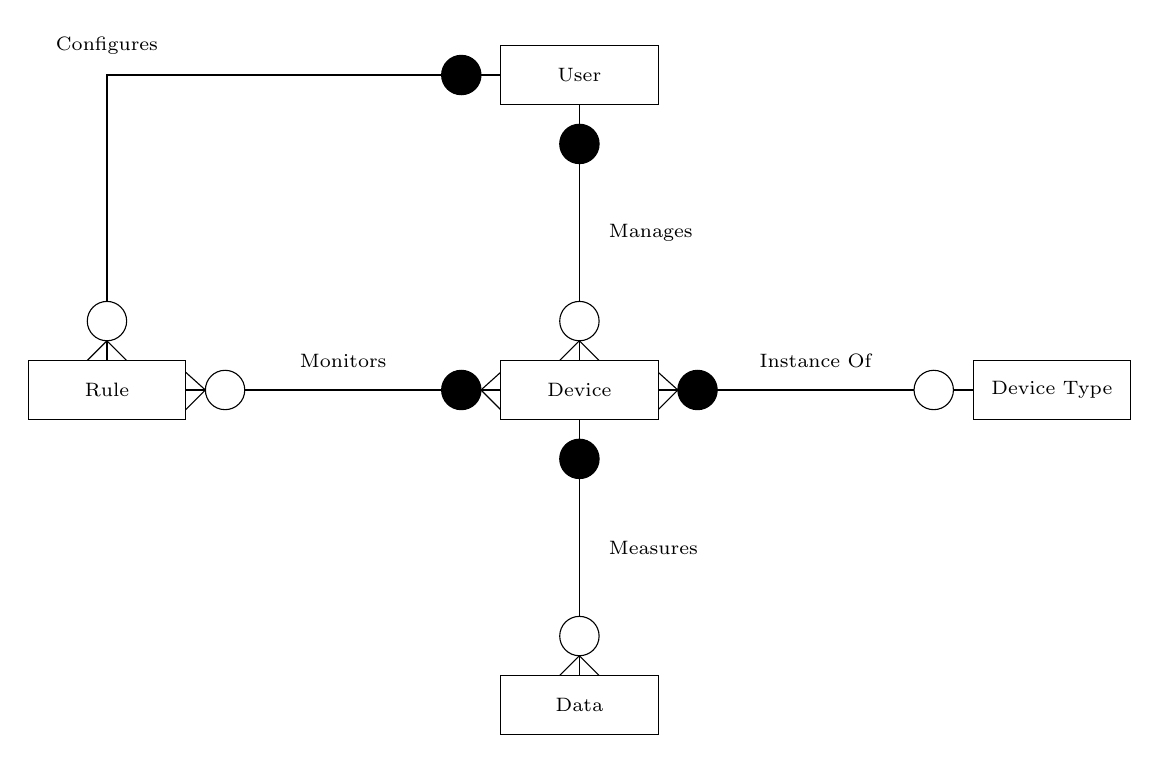
\begin{tikzpicture}
            \tikzstyle{every node}=[font=\scriptsize]

            \draw (7,8) -- (7,0.75);
            \draw (2,4.375) -- (12,4.375);
            \draw (1,4.75) -- (1,8.375) -- (6,8.375);

            \draw[fill=white] (2.5,4.375) circle [radius=0.25];
            \draw (2,4.6) -- (2.25, 4.375) -- (2,4.125);
            \node at (4,4.75) {Monitors};
            \draw (6,4.6) -- (5.75, 4.375) -- (6,4.125);
            \draw[fill=black] (5.5,4.375) circle [radius=0.25];

            \draw[fill=black] (8.5,4.375) circle [radius=0.25];
            \draw (8,4.6) -- (8.25, 4.375) -- (8,4.125);
            \node at (10,4.75) {Instance Of};
            \draw[fill=white] (11.5,4.375) circle [radius=0.25];

            \draw[fill=white] (7,5.25) circle [radius=0.25];
            \node[anchor=west] at (7.25,6.375) {Manages};
            \draw (6.75,4.75) -- (7, 5) -- (7.25,4.75);
            \draw[fill=black] (7,7.5) circle [radius=0.25];

            \draw[fill=black] (7,3.5) circle [radius=0.25];
            \node[anchor=west] at (7.25,2.375) {Measures};
            \draw (6.75,0.75) -- (7, 1) -- (7.25,0.75);
            \draw[fill=white] (7,1.25) circle [radius=0.25];

            \draw[fill=black] (5.5,8.375) circle [radius=0.25];
            \node at (1,8.75) {Configures};
            \draw (0.75,4.75) -- (1, 5) -- (1.25,4.75);
            \draw[fill=white] (1,5.25) circle [radius=0.25];

            \draw (0,4) rectangle (2,4.75);
            \node at (1,4.375) {Rule};

            \draw (6,0) rectangle (8,0.75);
            \node at (7,0.375) {Data};

            \draw (12,4) rectangle (14,4.75);
            \node at (13,4.375) {Device Type};

            \draw[fill=white] (6,4) rectangle (8,4.75);
            \node at (7,4.375) {Device};

            \draw (6,8) rectangle (8,8.75);
            \node at (7,8.375) {User};

          \end{tikzpicture}
        \caption{Entity Relationship Diagram for the Haar Engine}\label{figure:principal-models}
      \end{figure}

      2. Entity Sets
      \begin{itemize}
        \item User(\underline{id}, username, password, role)
        \item Device(\underline{id})
        \item Device Type(\underline{id}, type, structure)
        \item Data(\underline{id}, values)
        \item Rule(\underline{id}, watch target, criteria, action target, action)
      \end{itemize}

      3. Relationships
      \begin{itemize}
        \item Manages --- User manages Device [1:m][m:o]
        \item Configures --- User configures Rule [1:m][m:o]
        \item Instance Of --- Device instance of Device Type [m:1][o:m]
        \item Measures --- Device measures Data [1:m][m:o]
        \item Monitors --- Rule monitors Device [m:1][o:m]
      \end{itemize}

      4. Constraints and Assumptions
      \begin{itemize}
        \item Device Type structure is an array of objects. Each object describes a possible measurement.
        \item The Device Type of a device will never change
      \end{itemize}
    \subsection{Database Connector}
    \label{section:database-connector}
      Efficient data storage is an important performance consideration. The requirements in Chapter \ref{Chapter:Specification} also state that application developers should have the ability to change the database type to suit their own application. The design solution arrived at for this requirement is a database connector API.

      The database connector API will provide a set of foundation methods for operating on principal models and data generated by devices. The framework will use a consistent programming interface and this will allow application developers to change the connector for one of their own design. In a more strictly-typed programming language, object-oriented constructs such as abstract classes or interfaces might be used to define class signatures. With JavaScript, programming techniques like function composition might be more appropriate. 

      Whilst the Haar Engine will provide the capability of changing the database connector, an `out of the box' connector will be provided. A NoSQL database fits the purpose of the framework better than an SQL-based database because the data stored could be of varying formats and structures. There are a variety of NoSQL databases available, which will be discussed in the implementation chapter.

    \subsection{Data Access API}
      There are a number of mature standards used for structured data access on the web, so this requirement of the project is about choosing the most appropriate. Two widely-used access standards are Simple Object Access Protocol (SOAP) and Representational State Transfer (REST). These standards also use data interchange formats such as eXtensible Mark-up Language (XML) or JavaScript Object Notation (JSON).

      A REST API was found to be a better fit than SOAP for the Haar Engine. The REST access operators integrate much easier with potential implementation technologies like Node.js and Express and it is a simpler standard to use. The JSON data interchange format is based on JavaScript object constructs so it naturally integrates with a JavaScript-based application.

      Authentication will have to be enforced by every component of the Haar Engine, including the Data Access API. One characteristic of REST APIs is that they are stateless, meaning no session data is stored server-side and that every request will have to be inspected for appropriate access permissions. Two authentication techniques which will be used are a username and password combination, as well as token-based authentication. Clients will first authenticate with their username and password and if accepted, the REST API will return a unique access token for use in subsequent requests.

    \subsection{Real-Time Event API}
      One main characteristic of IoT is the ability to react on sensor data in real-time. This makes a robust and effective real-time API a priority for any given application. Giving structured access to this feature is challenging due to the points described in Section \ref{bidirectioncomms}. For this reason, the problem has been divided into two constituent components: opening and maintaining a true bidirectional communication channel, and efficiently handling messages between the two nodes of the channel.

      One technology which goes some distance in helping with this is MQTT. As described in Section \ref{section:mqtt}, MQTT is a publish-subscribe protocol which facilitates the transmission of messages. MQTT is a very robust protocol however given project constraints and additional the additional complexity which it might create, it has been deemed unfeasible for this project. Instead, the JavaScript project Socket.io can open and maintain WebSocket connections, with fallbacks if the WebSocket protocol is unavailable. The message-passing concepts of MQTT could be applied to Socket.io.

      \subsubsection{Connection Manager}
        The connection manager is responsible for navigating potential network issues to maintain a bidirectional communication channel. Choosing to use Socket.io and the WebSocket protocol should alleviate any of the issues regarding firewalls and NAT. Socket.io provides an API for managing WebSocket connections. Clients can connect to namespaced URIs which encapsulate different categories of client---the Haar Engine will use two default namespaces: sensors and actuators.

        It is also the responsibility of the connection manager to authenticate clients, whether they are users or devices. Socket.io also solves this problem with the use of its own middleware capability. This middleware could make use of authentication mechanisms already in place for the Data Access API.

      \subsubsection{Stream Processor}
        Once a connection has been established, it is the responsibility of the stream processor to act on messages. The Socket.io API allows clients to join one or more rooms within a given namespace and this capability will be leveraged by the stream processor. For example, multiple sensors will each have their own room under the sensor namespace. The stream processor can listen for any sensor events and store the data. Alternatively, stream processing rules (based on the rule principal object) could listen for messages in a single sensor room and act accordingly.

  \section{Haar}
    The main purpose of the second component, Haar, is to validate the implementation of the Haar Engine. Most of the heavy lifting will be done by the Haar Engine, however this application also requires design attention, especially in regards to the end devices. There are three main components to be investigated: the back-end application, front-end application (dashboard) and the wireless sensor network itself. Figure x.x. illustrates the relationship between these components.

    \subsection{Back-End Application}
      The back-end application is simply an instance of the Haar Engine. It is expected that the data models will be extended for one or two application-specific fields (such as a profile picture and biography for users) however it will generally be left as designed. The back-end application will be self-contained and separate from the front-end application. 

    \subsection{Front-End Application}
      The front-end application is, in essence, simply a user interface for the back-end APIs. It will make use of the Data Access API and Real-Time Event API to manage users, devices, rules and the authentication for all of them. The main challenge presented by the dashboard is handling very dynamic, real-time data in a structured and efficient way for a variety web browsers. The implementation details of this will be discussed in detail as part of the next chapter.

      What can be discussed at this stage is the design, layout and behaviour of the user interface. Figure \ref{figure:desktop-layout} illustrates the general layout which will be used. On desktop-sized web browsers, the window will be split into two panes---one used for navigation, and one for displaying the current page content. On mobile-sized web browsers, only one pane will be displayed at a time. By default, this will be the content pane and when the navigation button is clicked, the navigation pane will be shown.

      The behaviour of the user interface is a challenging aspect. It is expected that aspects of the user interface will react in real-time to new data, so it will also have to open a connection to the Real-Time Event API. This will be possible by using the Socket.io library client-side. The challenges begin when the user starts to navigate to different pages of the dashboard. Traditionally this would load a completely new page, however real-time connections would have to be renegotiated and this is inefficient. Instead, dashboard pages will be loaded asynchronously. Care must then be taken to achieving this in a structured way with in its implementation.

      \begin{figure}
        \centering
          \begin{tikzpicture}
            \node[inner sep=0pt] at (0,0)
              {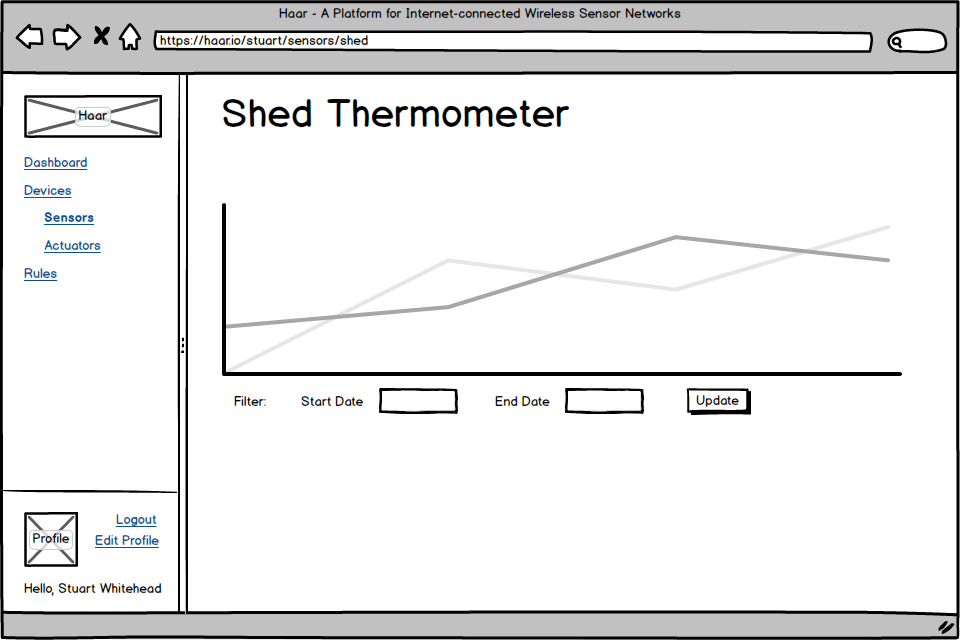
\includegraphics[width=\textwidth]{assets/desktop-layout.png}};
          \end{tikzpicture}
        \caption{UI layout for desktop-sized web browsers}\label{figure:desktop-layout}
      \end{figure}

    \subsection{Wireless Sensor Networks}
      The third and final component for the Haar application is the wireless sensor network. The wireless sensor network comprises of the physical sensors and actuators which create an interface between the physical and digital worlds. To fully demonstrate the capability of the Haar Engine, there is a requirement for a variety of sensor types.

      \subsubsection{Bridge}
        % Maintain communication channel
        % Map messages to and from nodes

      \subsubsection{End Devices}
        % Low-power nodes
        % Constrained processing power